\setcounter{page}{3}
\chapter{Задание}


\begin{enumerate}
	\item Для выборки объема $n$ из нормальной генеральной совокупности $X$ реализовать в виде программы на ЭВМ
	\begin{enumerate}
		\item вычисление точечных оценок $\hat\mu(\vec x_n)$ и $S^2(\vec x_n)$ математического ожидания $MX$ и дисперсии $DX$ соответственно;
		\item вычисление нижней и верхней границ $\underline\mu(\vec x_n)$, $\overline\mu(\vec x_n)$ для $\gamma$-доверительного интервала для математического ожидания $MX$;
		\item вычисление нижней и верхней границ $\underline\sigma^2(\vec x_n)$, $\overline\sigma^2(\vec x_n)$ для $\gamma$-доверительного интервала для дисперсии $DX$;
	\end{enumerate}
	\item вычислить $\hat\mu$ и $S^2$ для выборки из индивидуального варианта;
	\item для заданного пользователем уровня доверия $\gamma$ и $N$ – объема выборки из индивидуального варианта:
	\begin{enumerate}
		\item на координатной плоскости $Oyn$ построить прямую $y = \hat\mu(\vec{x_N})$, также графики функций $y = \hat\mu(\vec x_n)$, $y = \underline\mu(\vec x_n)$ и $y = \overline\mu(\vec x_n)$ как функций объема $n$ выборки, где $n$ изменяется от 1 до $N$;
		\item на другой координатной плоскости $Ozn$ построить прямую $z = S^2(\vec{x_N})$, также графики функций $z = S^2(\vec x_n)$, $z = \underline\sigma^2(\vec x_n)$ и $z = \overline\sigma^2(\vec x_n)$ как функций объема $n$ выборки, где $n$ изменяется от 1 до $N$.
	\end{enumerate}
\end{enumerate}


Данные для лабораторной работы по индивидуальному варианту:

\begin{lstlisting}
X = [-8.47, -7.45, -7.12, -8.30, -8.15, -6.01, -5.20, -7.38, -6.76, -9.18, -6.00, -8.08, -7.96, -8.34, -6.82, -8.46, -8.07, -7.04, -7.24, -8.16, -8.20, -8.27, -7.79, -7.37, -7.02, -7.13, -6.99, -7.65, -8.18, -6.71, -8.41, -6.71, -7.04, -9.15, -7.74, -10.11, -8.20, -7.07, -7.63, -8.99, -6.62, -6.23, -7.13, -6.41, -7.06, -7.72, -8.44, -8.85, -8.02, -6.98, -6.08, -7.20, -7.48, -7.82, -9.19, -8.31, -7.95, -7.97, -6.66, -6.59, -9.10, -7.87, -9.02, -8.77, -7.62, -9.44, -8.05, -7.60, -7.33, -6.94, -8.51, -7.39, -6.44, -8.88, -8.21, -7.66, -6.91, -8.39, -7.37, -7.26, -6.04, -7.58, -7.28, -7.02, -7.10, -7.33, -8.63, -8.21, -7.12, -8.11, -9.03, -8.11, -8.79, -9.22, -7.32, -5.97, -7.26, -6.39, -7.64, -8.38, -7.67, -7.70, -7.70, -8.95, -6.25, -8.09, -7.85, -8.10, -7.73, -6.78, -7.78, -8.20, -8.88, -8.51, -7.45, -7.14, -6.63, -7.38, -7.72, -6.25]
\end{lstlisting}

\chapter{Теоретическая часть}

\section{Теоретические сведения}

\subsection{Интервальные оценки}

Пусть X --- случайная величина, закон распределения которой известен с точностью до неизвестного параметра $\theta$. 

Интервальной оценкой параметра $\theta$ уровня $\gamma$ ($\gamma$-интервальной оценкой) называют пару статистик $\underline{\theta}(\vec X) \text{ и } \overline{\theta}(\vec X)$ таких, что $$P\{\theta \in (\underline{\theta}(\vec X), \overline{\theta}(\vec X))\}=\gamma$$ 

$\gamma$-доверительным интервалом (доверительным интервалом уровня $\gamma$) для параметра $\theta$ называют реализацию (выборочное значение) интервальной оценки уровня $\gamma$ для этого параметра.

\subsection{Вычисление границ доверительных интервалов}

Формулы для вычисления границ $\gamma$-доверительного интервала для математического ожидания нормальной случайной величины:

$$
\underline\mu(\vec X_n)=\overline X - \frac{S(\vec X)t^{(n-1)}_{\frac{1+\gamma}{2}}}{\sqrt{n}},
$$

$$
\overline\mu(\vec X_n)=\overline X + \frac{S(\vec X)t^{(n-1)}_{\frac{1+\gamma}{2}}}{\sqrt{n}},
$$
где $\overline X$ --- выборочное среднее, $S^2(\vec X)$ --- исправленная выборочная дисперсия, $t^{(n-1)}_{\alpha}$ --- квантиль уровня $\alpha$ распределения Стьюдента с $n-1$ степенями свободы.

Формулы для вычисления границ $\gamma$-доверительного интервала для дисперсии нормальной случайной величины:

$$
\underline\sigma^2(\vec X_n)= \frac{(n-1)S^2(\vec X)}{h^{(n-1)}_{\frac{1+\gamma}{2}}},
$$

$$
\overline\sigma^2(\vec X_n)= \frac{(n-1)S^2(\vec X)}{h^{(n-1)}_{\frac{1-\gamma}{2}}},
$$
где $S^2(\vec X)$ --- исправленная выборочная дисперсия, $h^{(n-1)}_{\alpha}$ --- квантиль уровня $\alpha$ распределения $\chi^2$ с $n - 1$ степенями свободы.

\chapter{Практическая часть}

\section{Код программы}

\begin{lstlisting}
x = [-8.47, -7.45, -7.12, -8.30, -8.15, -6.01, -5.20, -7.38, -6.76, -9.18, -6.00, -8.08, -7.96, -8.34, -6.82, -8.46, -8.07, -7.04, -7.24, -8.16, -8.20, -8.27, -7.79, -7.37, -7.02, -7.13, -6.99, -7.65, -8.18, -6.71, -8.41, -6.71, -7.04, -9.15, -7.74, -10.11, -8.20, -7.07, -7.63, -8.99, -6.62, -6.23, -7.13, -6.41, -7.06, -7.72, -8.44, -8.85, -8.02, -6.98, -6.08, -7.20, -7.48, -7.82, -9.19, -8.31, -7.95, -7.97, -6.66, -6.59, -9.10, -7.87, -9.02, -8.77, -7.62, -9.44, -8.05, -7.60, -7.33, -6.94, -8.51, -7.39, -6.44, -8.88, -8.21, -7.66, -6.91, -8.39, -7.37, -7.26, -6.04, -7.58, -7.28, -7.02, -7.10, -7.33, -8.63, -8.21, -7.12, -8.11, -9.03, -8.11, -8.79, -9.22, -7.32, -5.97, -7.26, -6.39, -7.64, -8.38, -7.67, -7.70, -7.70, -8.95, -6.25, -8.09, -7.85, -8.10, -7.73, -6.78, -7.78, -8.20, -8.88, -8.51, -7.45, -7.14, -6.63, -7.38, -7.72, -6.25];

gamma = input("gamma > ")

n = length(x);

mu = sum(x) / n
s2 = sum((x - mu) .^ 2) / (n - 1)

mu_min = mu - sqrt(s2) * tinv((1 + gamma) / 2, n - 1) / sqrt(n)
mu_max = mu + sqrt(s2) * tinv((1 + gamma) / 2, n - 1) / sqrt(n)

s2_min = s2 * (n - 1) / chi2inv((1 + gamma) / 2, n - 1)
s2_max = s2 * (n - 1) / chi2inv((1 - gamma) / 2, n - 1)

ns = zeros(1, n);

mus = zeros(1, n);
mu_mins = zeros(1, n);
mu_maxes = zeros(1, n);

s2s = zeros(1, n);
s2_mins = zeros(1, n);
s2_maxes = zeros(1, n);

mu_const = zeros(1, n);
s2_const = zeros(1, n);

for i = 1:n
    ns(i) = i;
    locx = x(1:i);

    mu_const(i) = mu;
    s2_const(i) = s2;

    mus(i) = sum(locx) / i;
    s2s(i) = sum((locx - mu) .^ 2) / (i - 1);

    mu_mins(i) = mus(i) - sqrt(s2s(i)) * tinv((1 + gamma) / 2, i - 1) / sqrt(i);
    mu_maxes(i) = mus(i) + sqrt(s2s(i)) * tinv((1 + gamma) / 2, i - 1) / sqrt(i);

    s2_mins(i) = (i - 1) * s2s(i) / chi2inv((1 + gamma) / 2, i - 1);
    s2_maxes(i) = (i - 1) * s2s(i) / chi2inv((1 - gamma) / 2, i - 1);
end

plot(ns, mu_const, ns, mus, ns, mu_mins, ns, mu_maxes, 'LineWidth', 1.5);
title('$\hat \mu$','interpreter','latex', 'FontSize', 14);
xlabel('n');
ylabel('y');
legend('$\hat \mu(\vec x_N)$', '$\hat \mu(\vec x_n)$', '$\underline{\mu}(\vec x_n)$', '$\overline{\mu}(\vec x_n)$', 'Interpreter', 'latex', 'FontSize', 14);

figure;

plot(ns, s2_const, ns, s2s, ns, s2_mins, ns, s2_maxes, 'LineWidth', 1.5);
title('$\hat S^2$','interpreter','latex', 'FontSize', 14);
xlabel('n');
ylabel('z');
legend('$\hat S^2(\vec x_N)$', '$\hat S^2(\vec x_n)$', '$\underline{\sigma}^2(\vec x_n)$', '$\overline{\sigma}^2(\vec x_n)$', 'Interpreter', 'latex', 'FontSize', 14);
\end{lstlisting}

\section{Результат работы программы}

\subsection{Числовые характеристики}
Для $\gamma = 0.9$:
\begin{equation*}
	\hat\mu(\vec x_N) = -7.6609\\
\end{equation*}
\begin{equation*}
	S^2(\vec x_N) = 0.7779\\
\end{equation*}
\begin{equation*}
	\underline\mu(\vec x_N) = -7.7944\\
\end{equation*}
\begin{equation*}
	\overline\mu(\vec x_N) = -7.5274 \\
\end{equation*}
\begin{equation*}
	\underline{S^2}(\vec x_N) = 0.6364\\
\end{equation*}
\begin{equation*}
	\overline{S^2}(\vec x_N) = 0.9764\\
\end{equation*}

\newpage

\subsection{Графики}

\begin{figure}[h!]
 \center{\includegraphics[width=0.7\textwidth]{images/1.png}}
 \caption{Графики $y = \hat\mu(\vec x_N)$, $y(n) = \hat\mu(\vec x_n)$, $y(n) = \underline\mu(\vec x_n)$, $y(n) = \overline\mu(\vec x_n)$}
\end{figure}

\begin{figure}[!h]
 \center{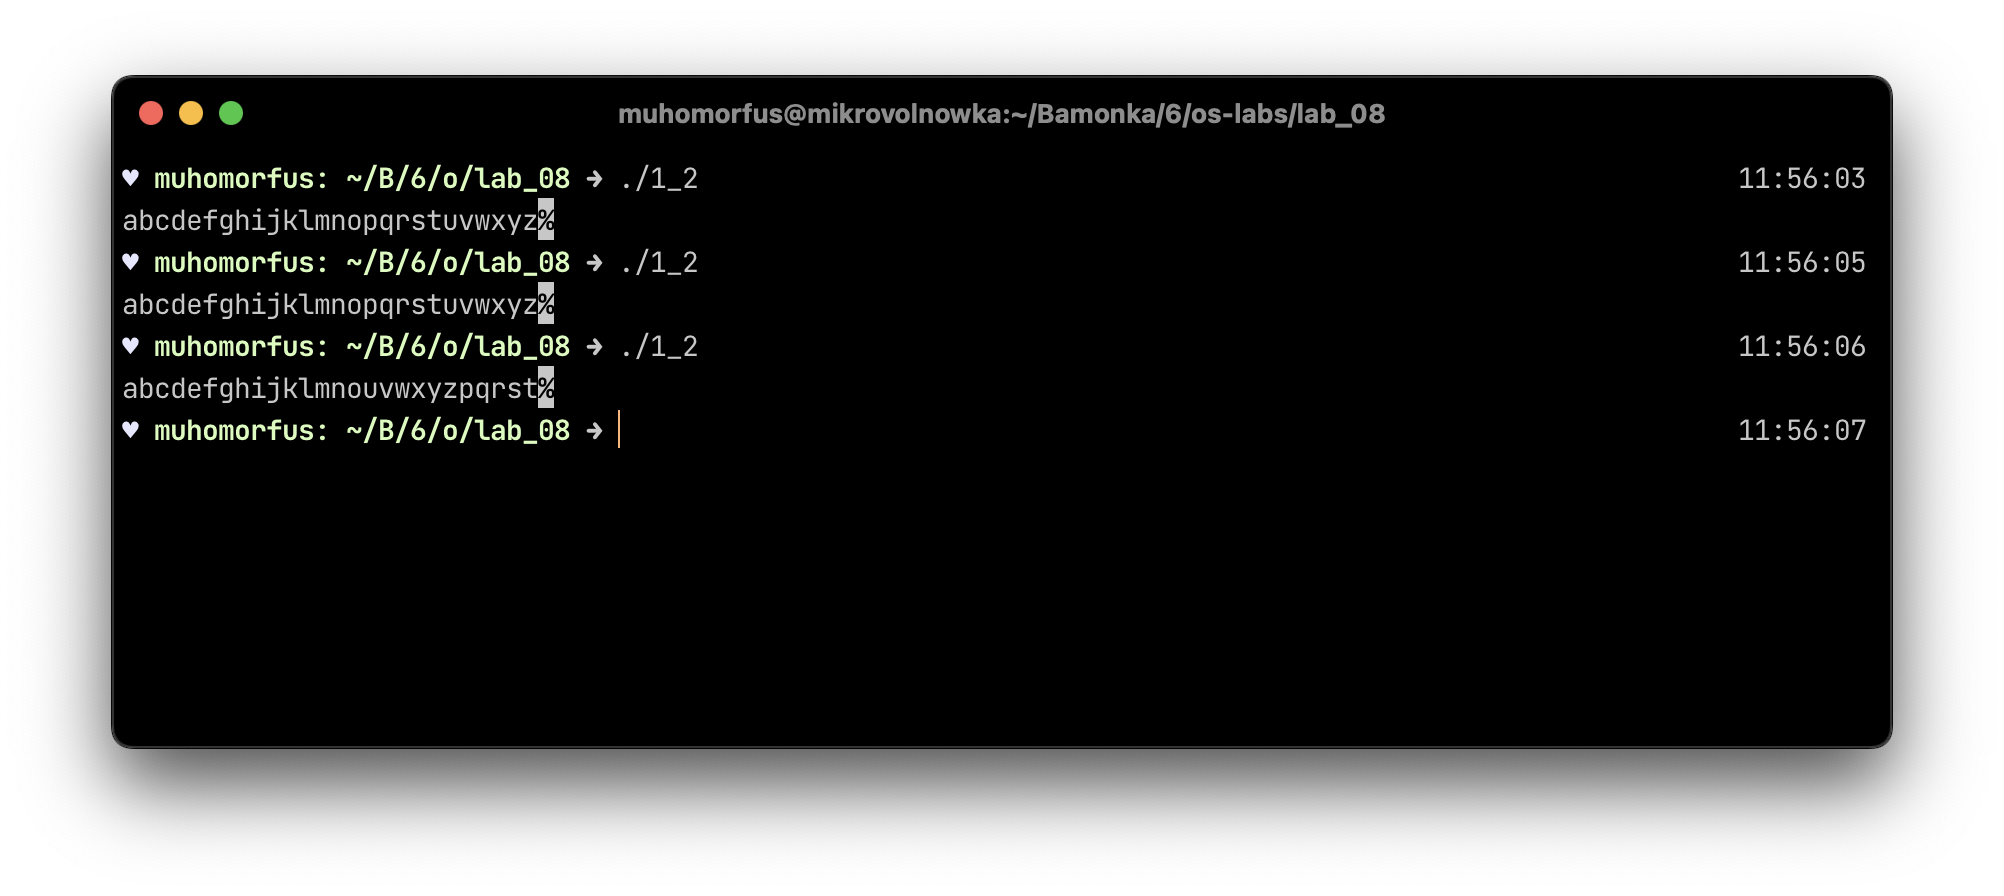
\includegraphics[width=0.7\textwidth]{images/2.png}}
 \caption{Графики $z = S^2(\vec x_N)$, $z(n) = S^2(\vec x_n)$, $z(n) = \underline \sigma^2(\vec x_n)$, $z(n) = \overline \sigma^2(\vec x_n)$}
\end{figure}

\newpage